\documentclass[a4paper]{report}
\usepackage[english]{babel}
\usepackage{amssymb}
\usepackage{amsmath}
\usepackage{graphicx}
\usepackage{float}
\usepackage{shortvrb}
\usepackage{cancel}
\usepackage[T1]{fontenc}
\usepackage{nicefrac}
\usepackage{amsfonts}
\usepackage{standalone} %Makes it possible to ignore other preambles of child document
\usepackage{eurosym} %Euro teken mogelijk
\usepackage{multirow} %For multiple rows togheter in one table
\usepackage{parskip} %For a small white line between paragraphs
\usepackage[protrusion=true,expansion=true]{microtype}
\usepackage{hyperref}%For automatic and URL Reference
\usepackage{appendix}
%Possible to change the margins
\usepackage{geometry}
\geometry{verbose,tmargin=1.9cm,bmargin=1.8cm,lmargin=2cm,rmargin=2cm}

\usepackage{subfig}

%include pdf pages
\usepackage{pdfpages}

%being able to create tables over multiple pages
\usepackage{longtable}

\makeatletter

%Change standard font size
\renewcommand\normalsize{ \@setfontsize\normalsize{11pt}{11pt}}\normalsize  
\makeatother

\usepackage{fancyhdr}
\pagestyle{fancy}
\fancyhead{}
\fancyfoot{}

%Gives text above each page
\fancyhead[CO,CE]{DSE Project}

%Page number
\fancyfoot[RO,LE]{\thepage}


\usepackage{babel}

%Available structures:
%Report: \part{}, \chapter{}, \section{}, \subsection{}, \subsubsection{}, \paragraph{}, \subparagraph{}

\begin{document}
\chapter{Work breakdown structure}

\begin{figure}
\label{fig:WBSFPP}
\centering
\includegraphics[height=20cm]{Figures/WBS_FPP.png}
\caption{performance and propulsion WBS tree}
\end{figure}

\begin{figure}
\label{fig:WBSA}
\centering
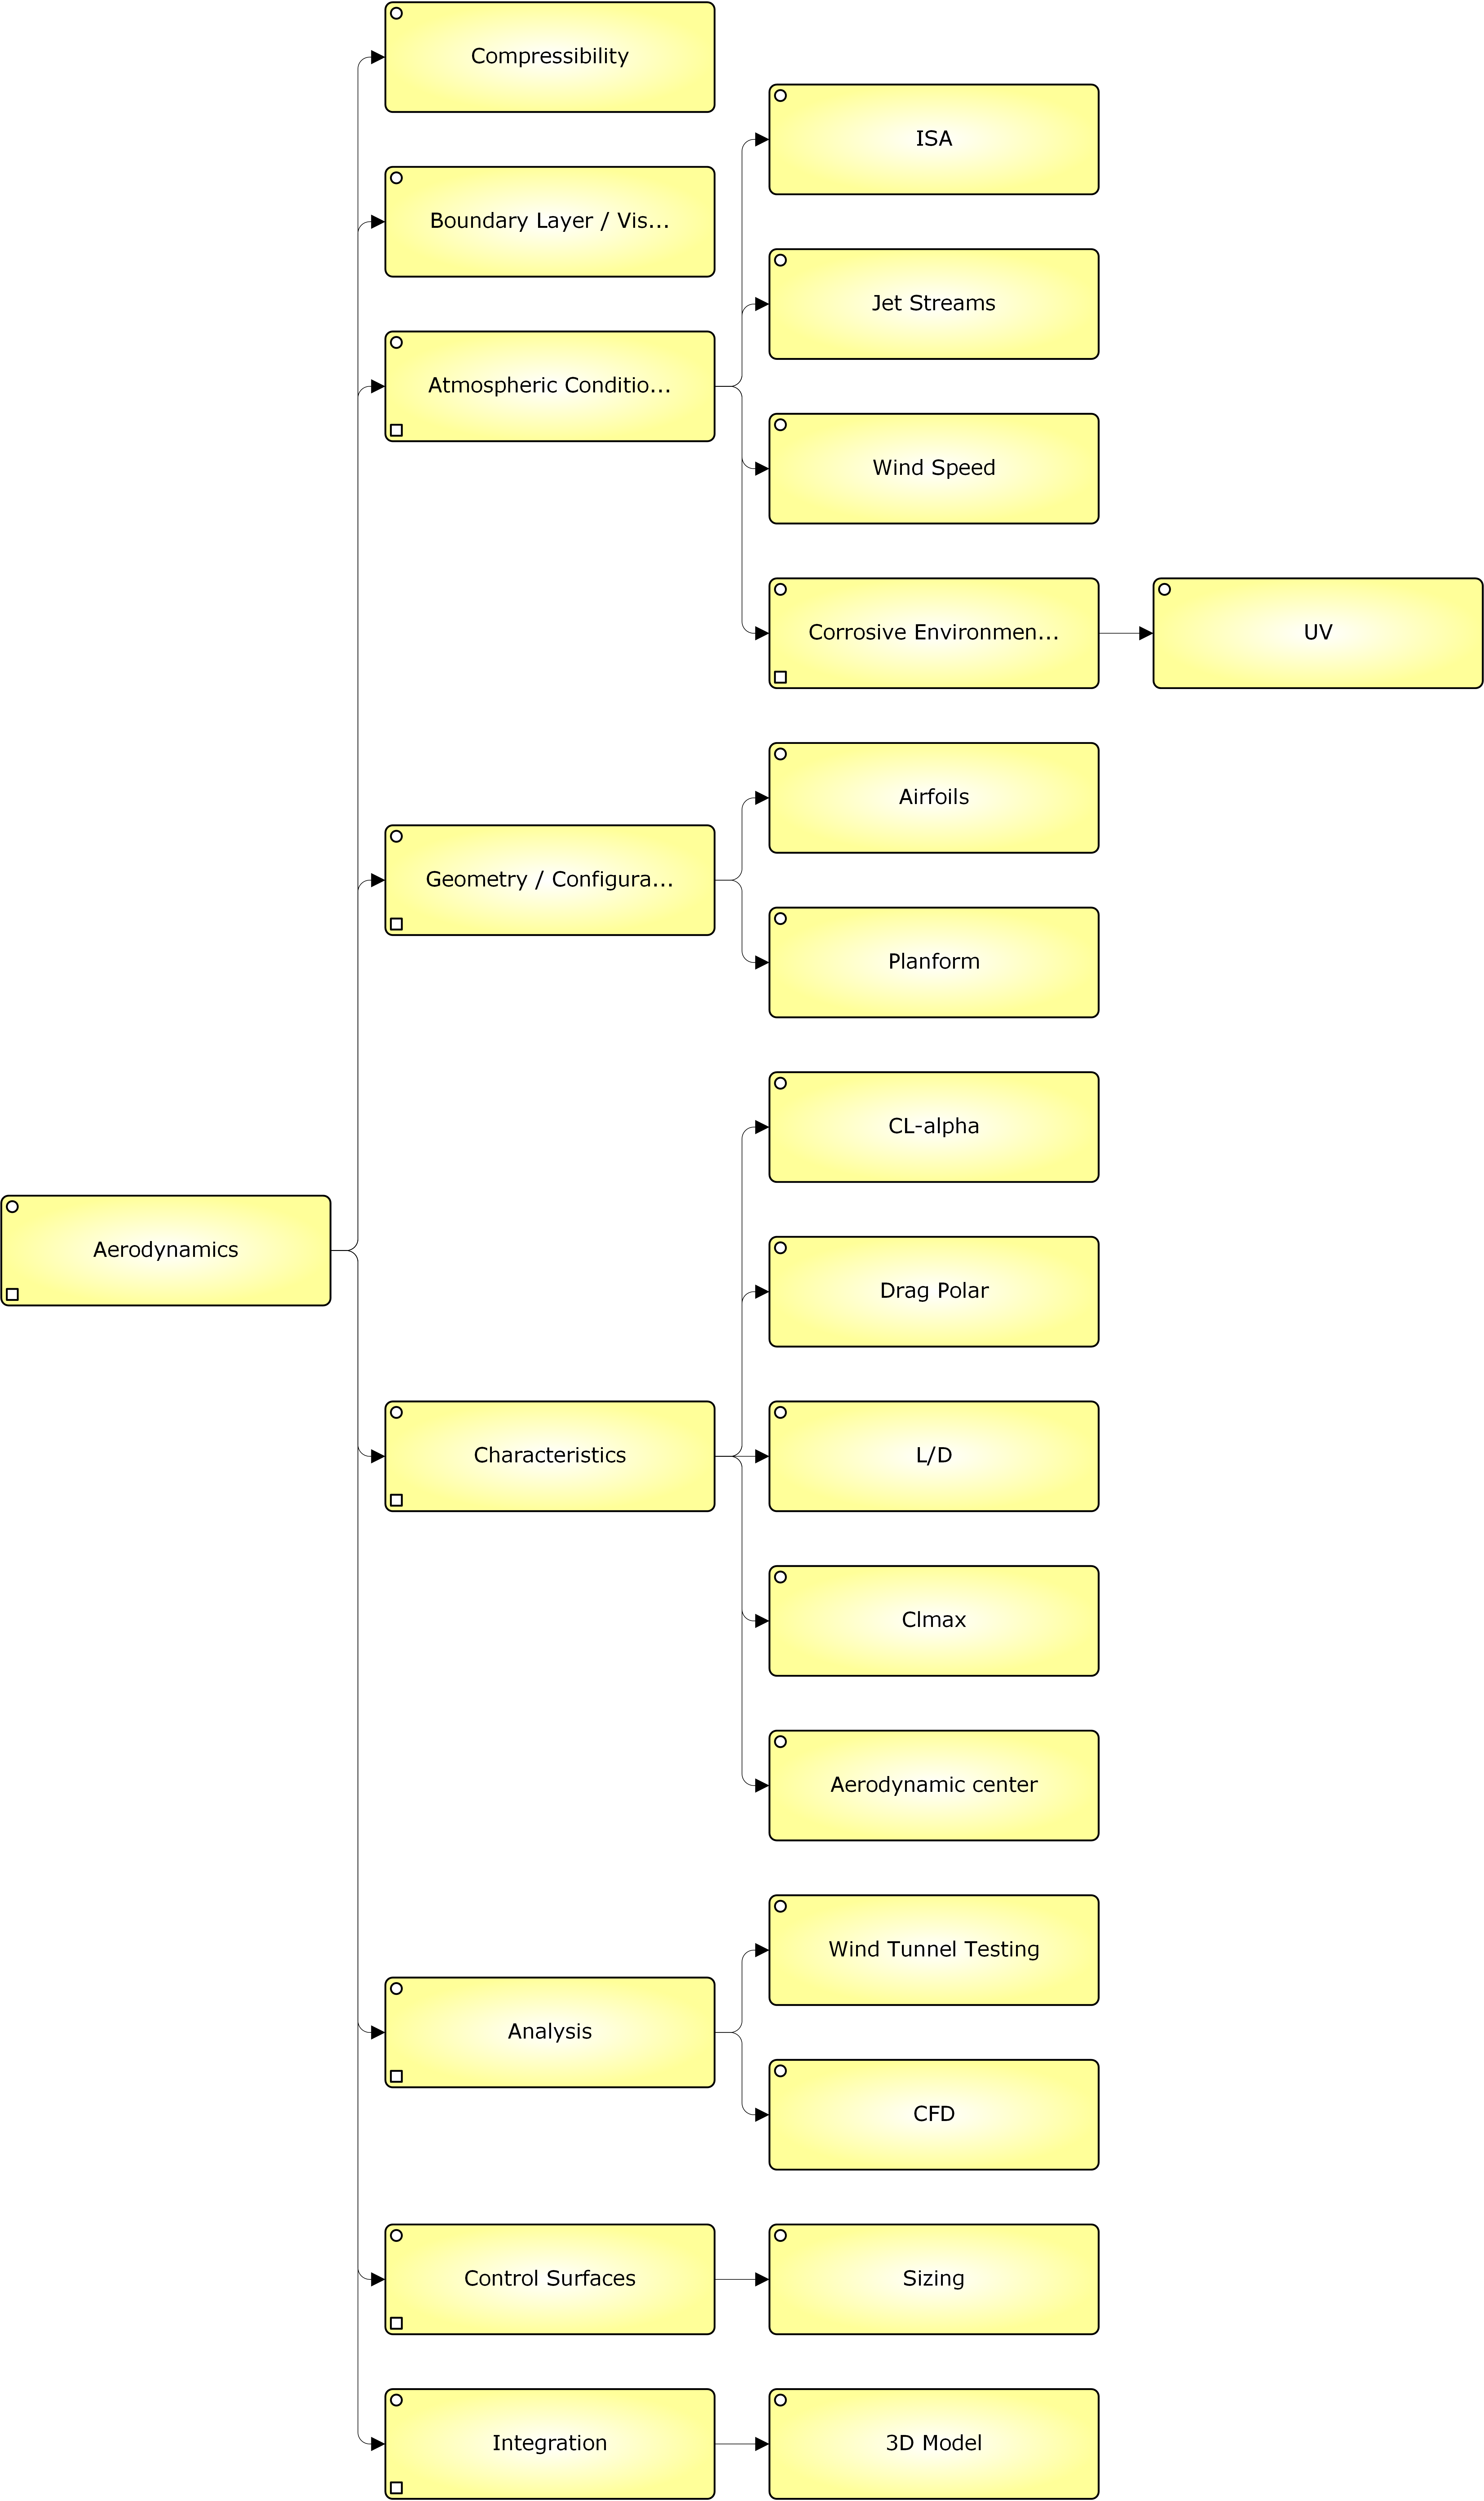
\includegraphics[height=20cm]{Figures/WBS_A.png}
\caption{Aerodynamics WBS tree}
\end{figure}



\begin{figure}
\label{fig:WBSSC}
\centering
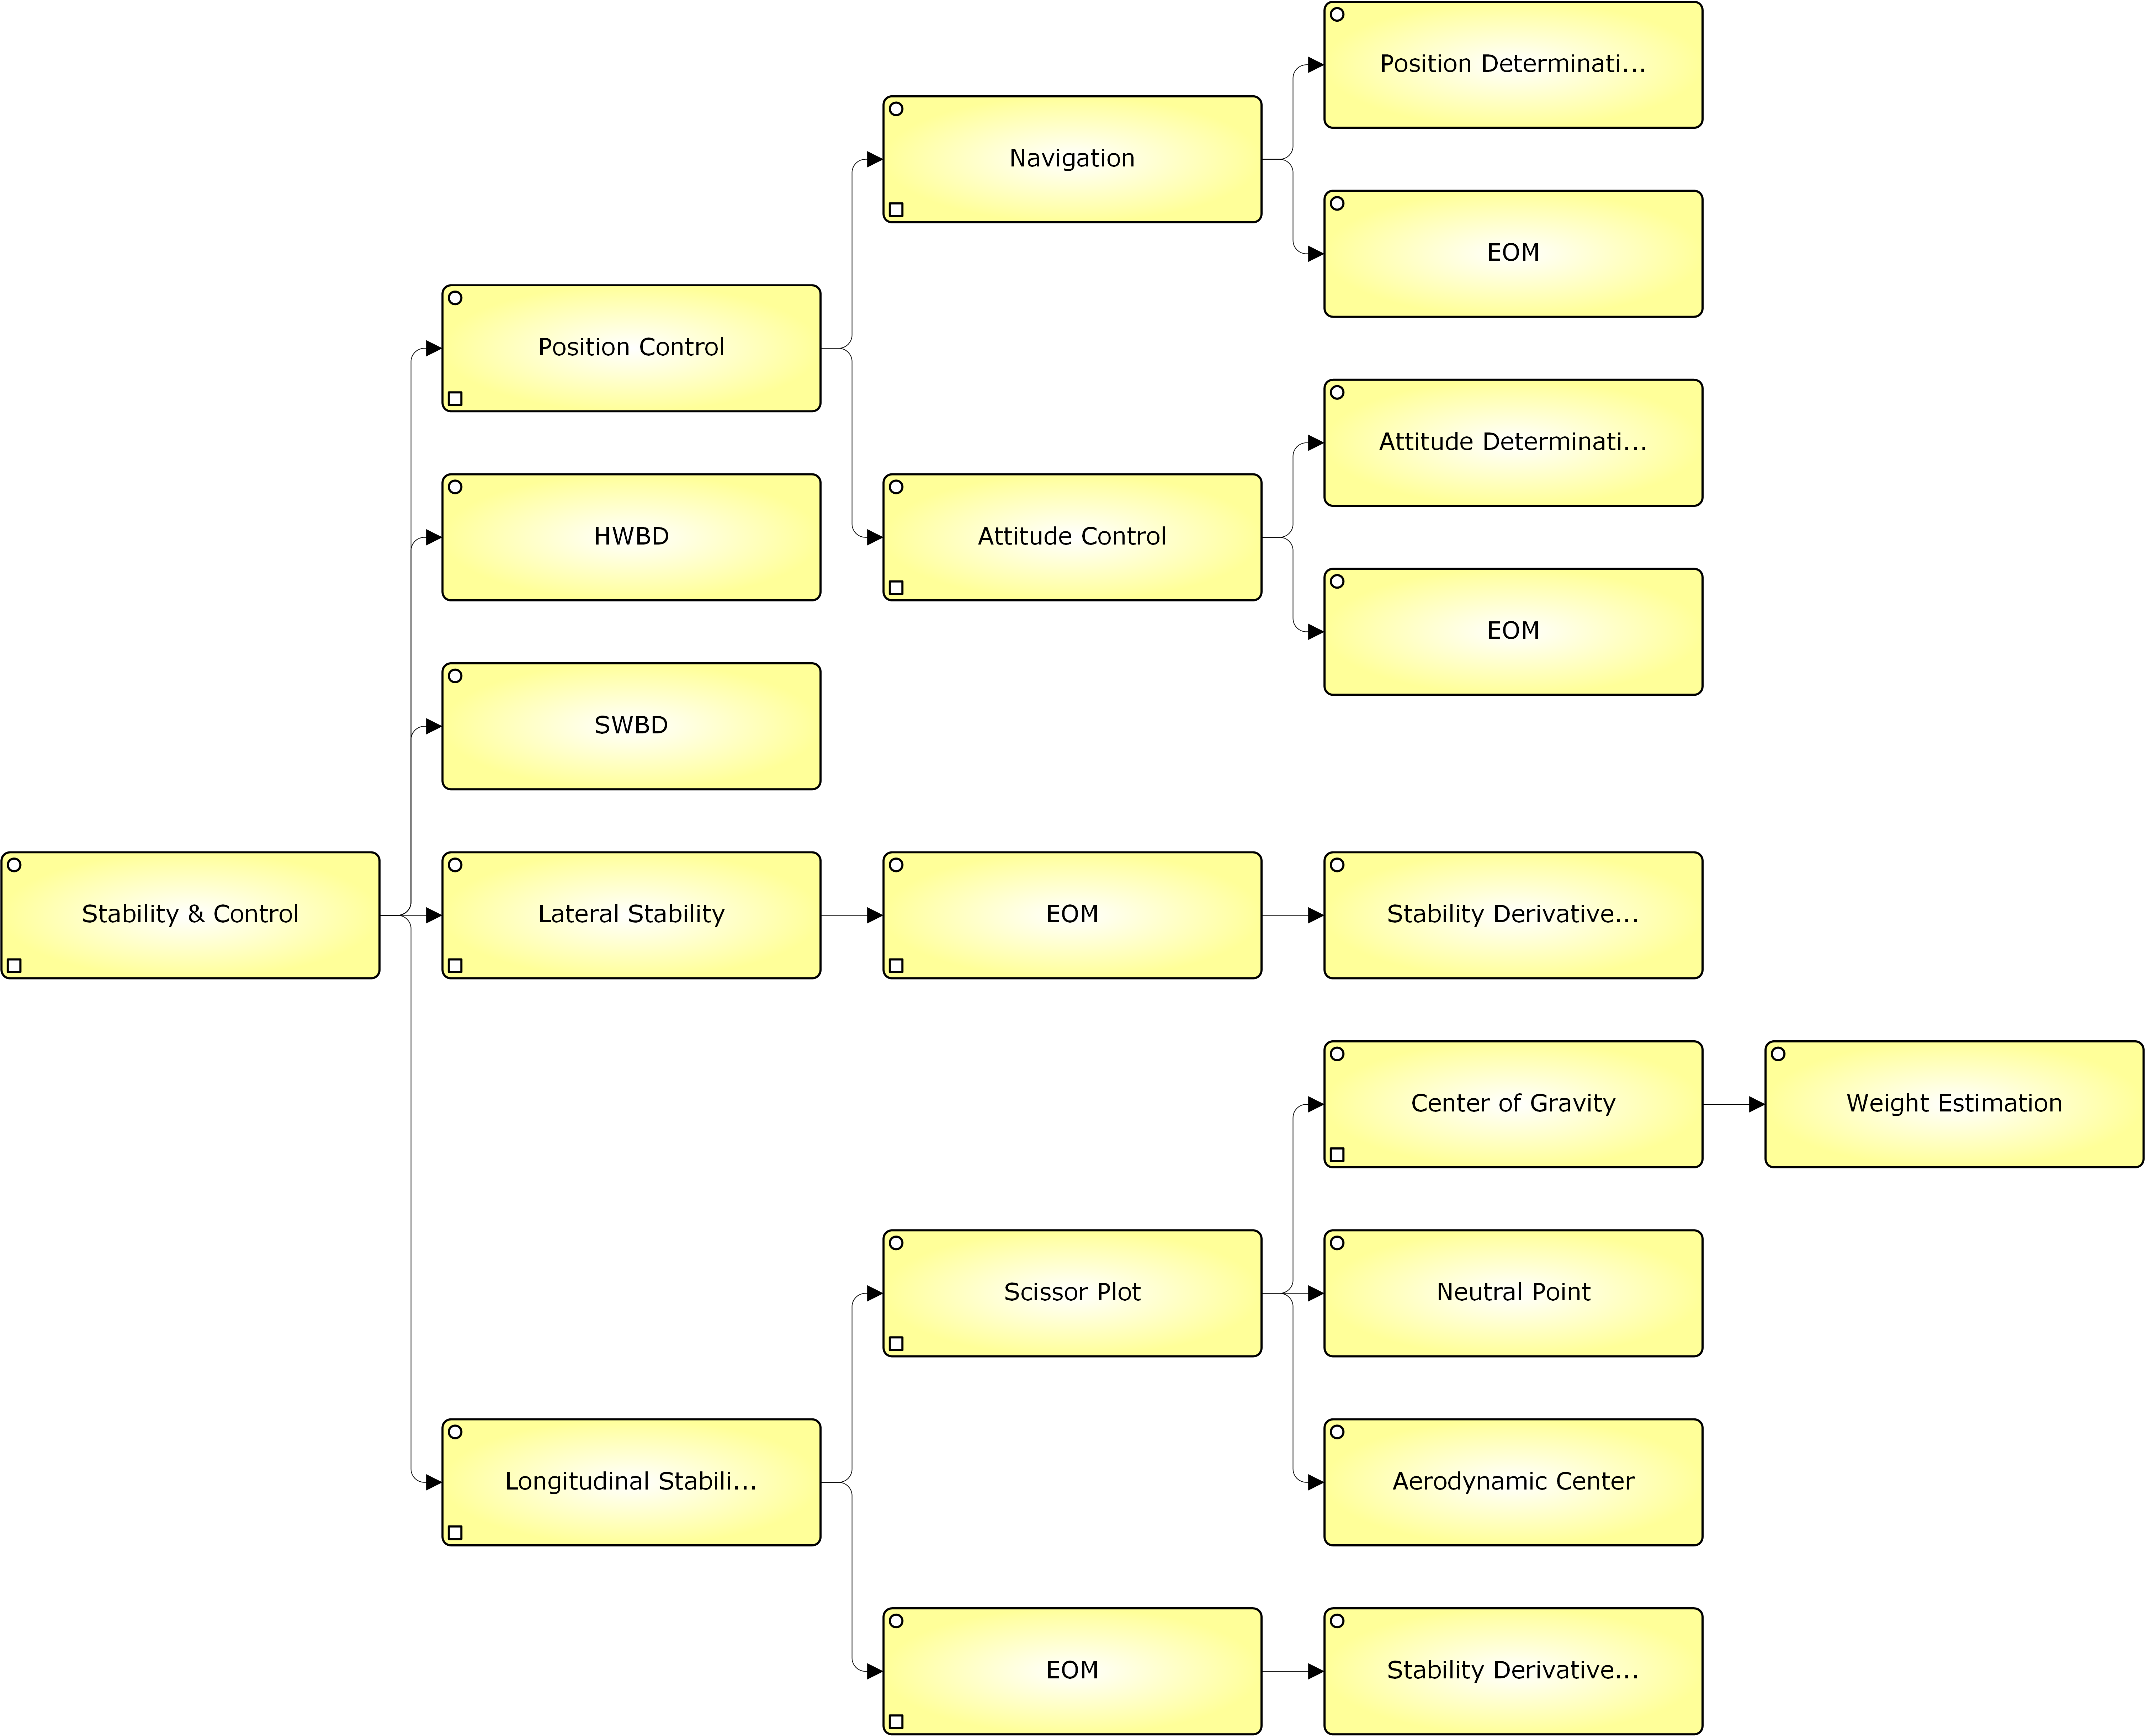
\includegraphics[width=\textwidth]{Figures/WBS_SC.png}

\caption{Stability and control WBS tree}
\end{figure}


\begin{figure}
\label{fig:WBSMS}
\centering
\includegraphics[height=20cm]{Figures/WBS_MS.png}

\caption{Materials and structural WBS tree}
\end{figure}



\begin{figure}
\label{fig:WBSPM}
\centering
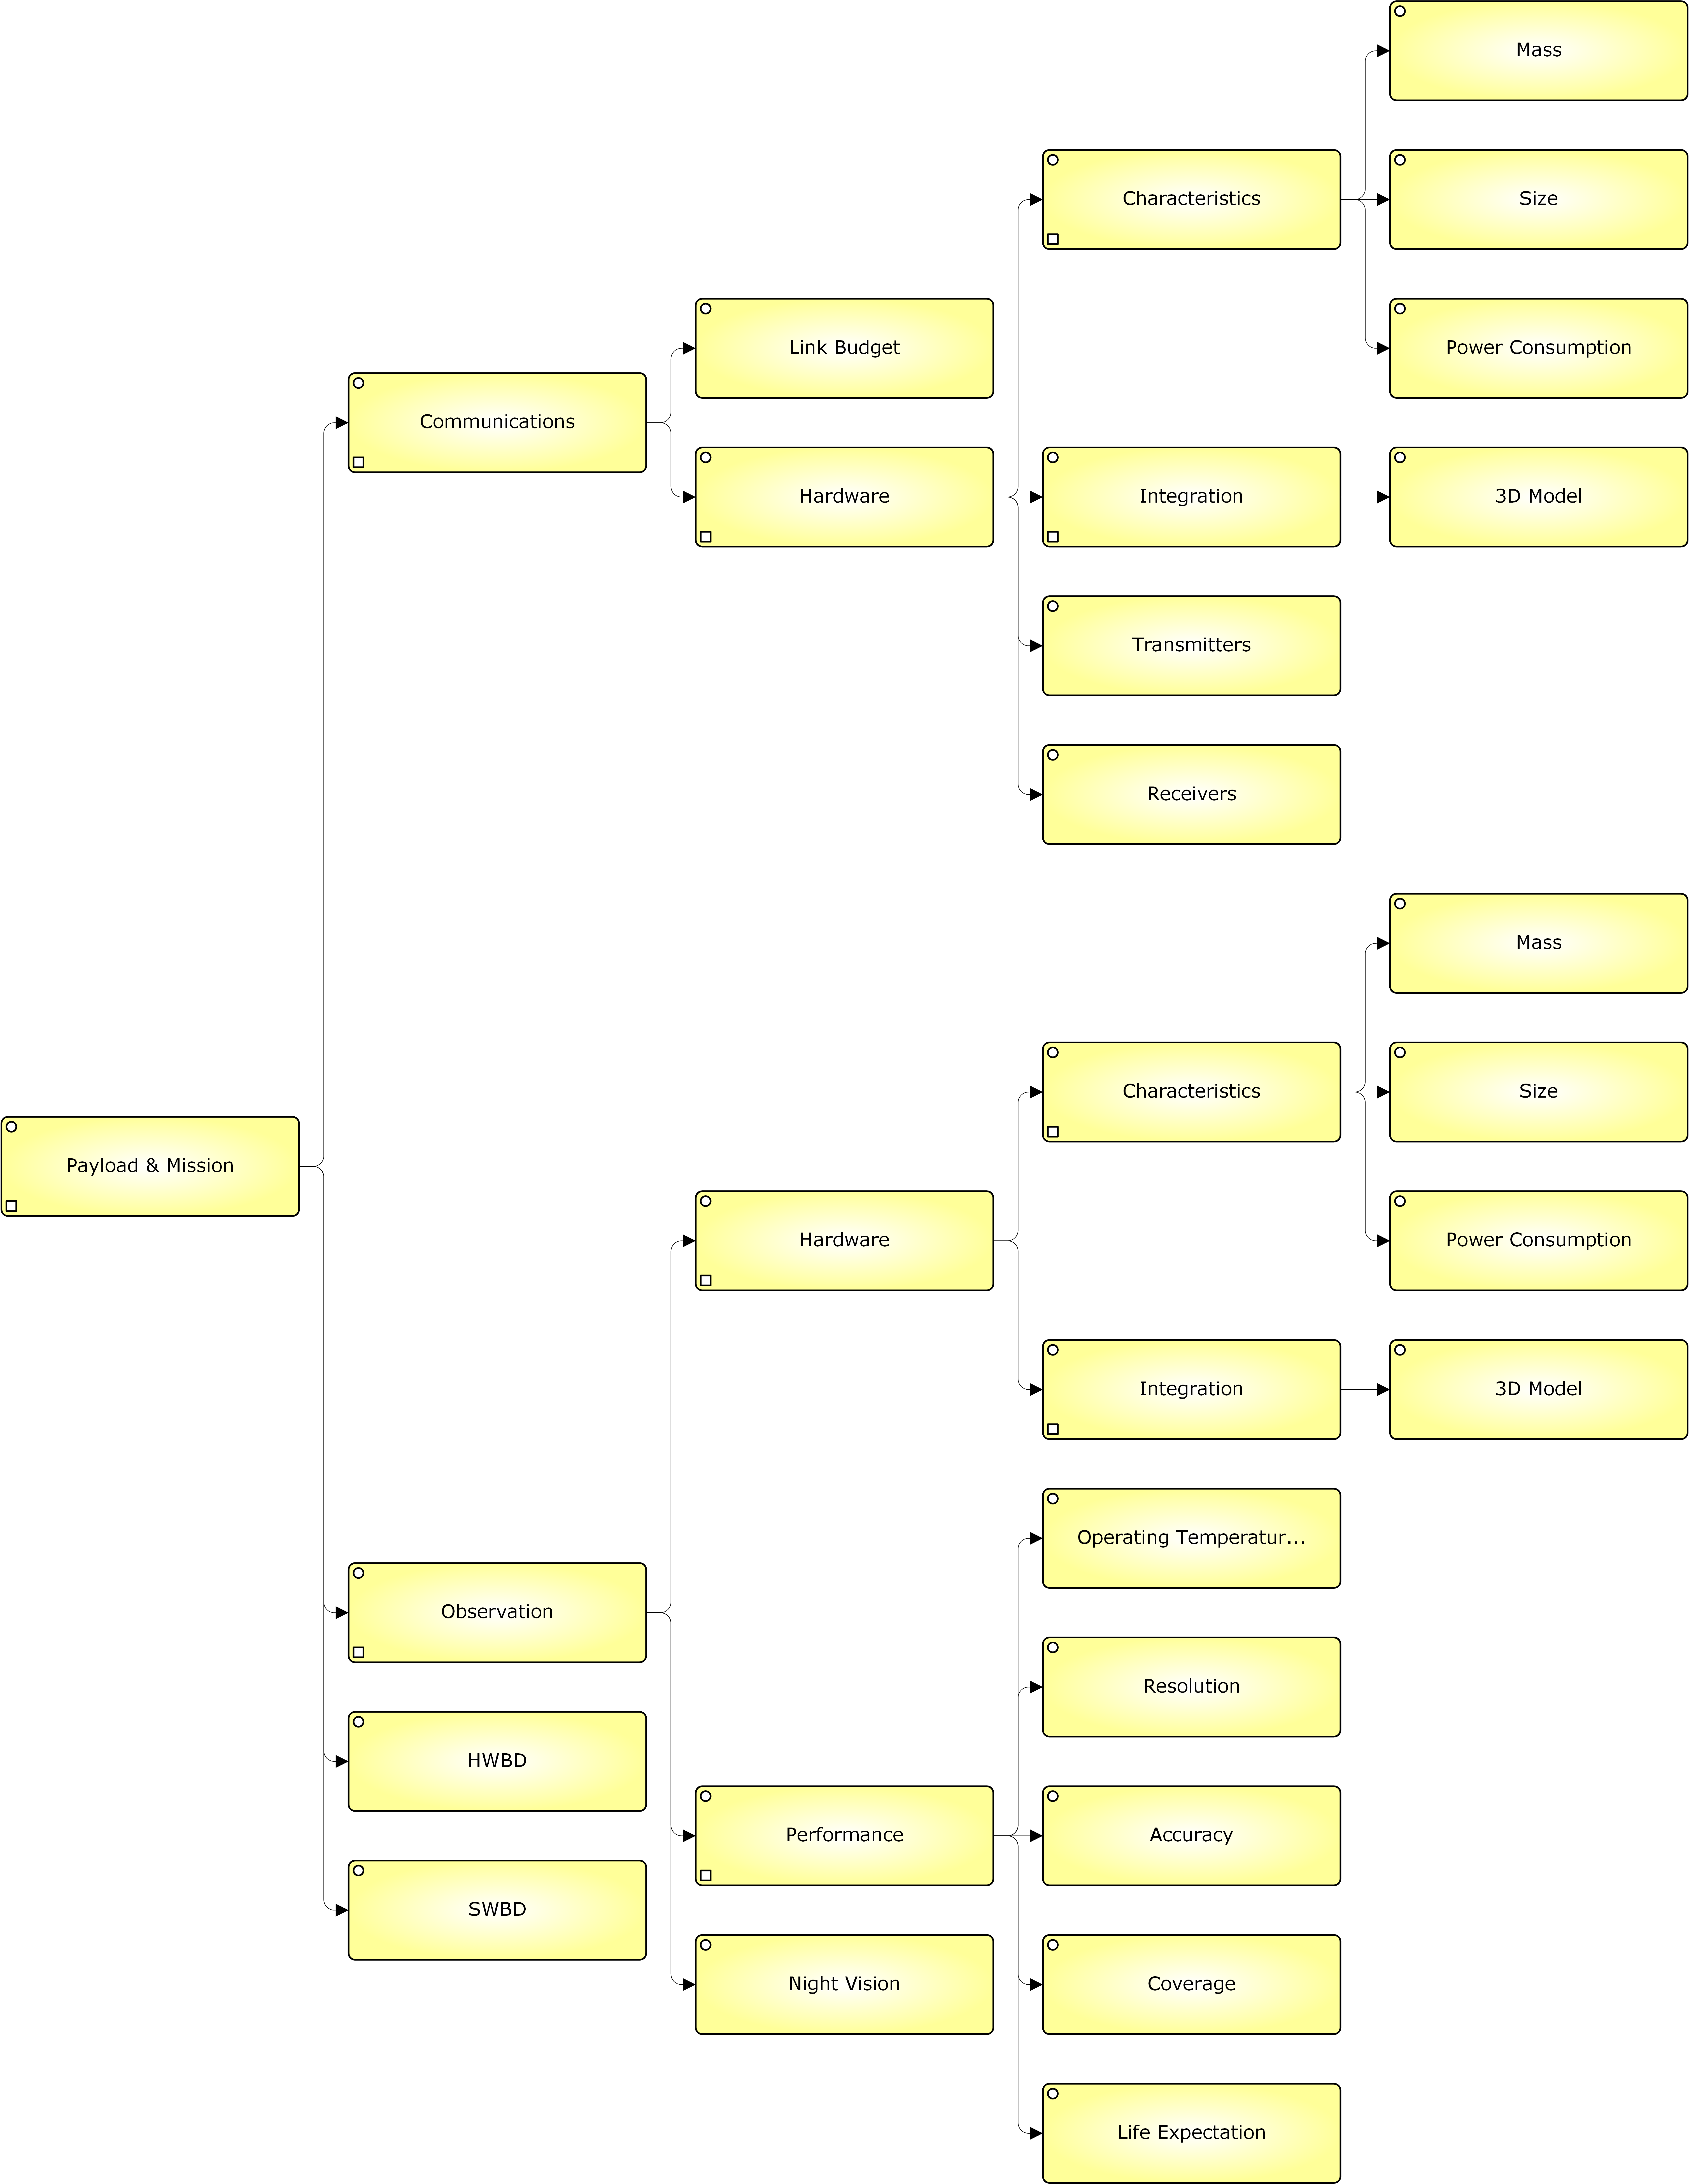
\includegraphics[height=20cm]{Figures/WBS_PM.png}

\caption{Payload and mission WBS tree}
\end{figure}


\begin{figure}
\label{fig:WBSO}
\centering
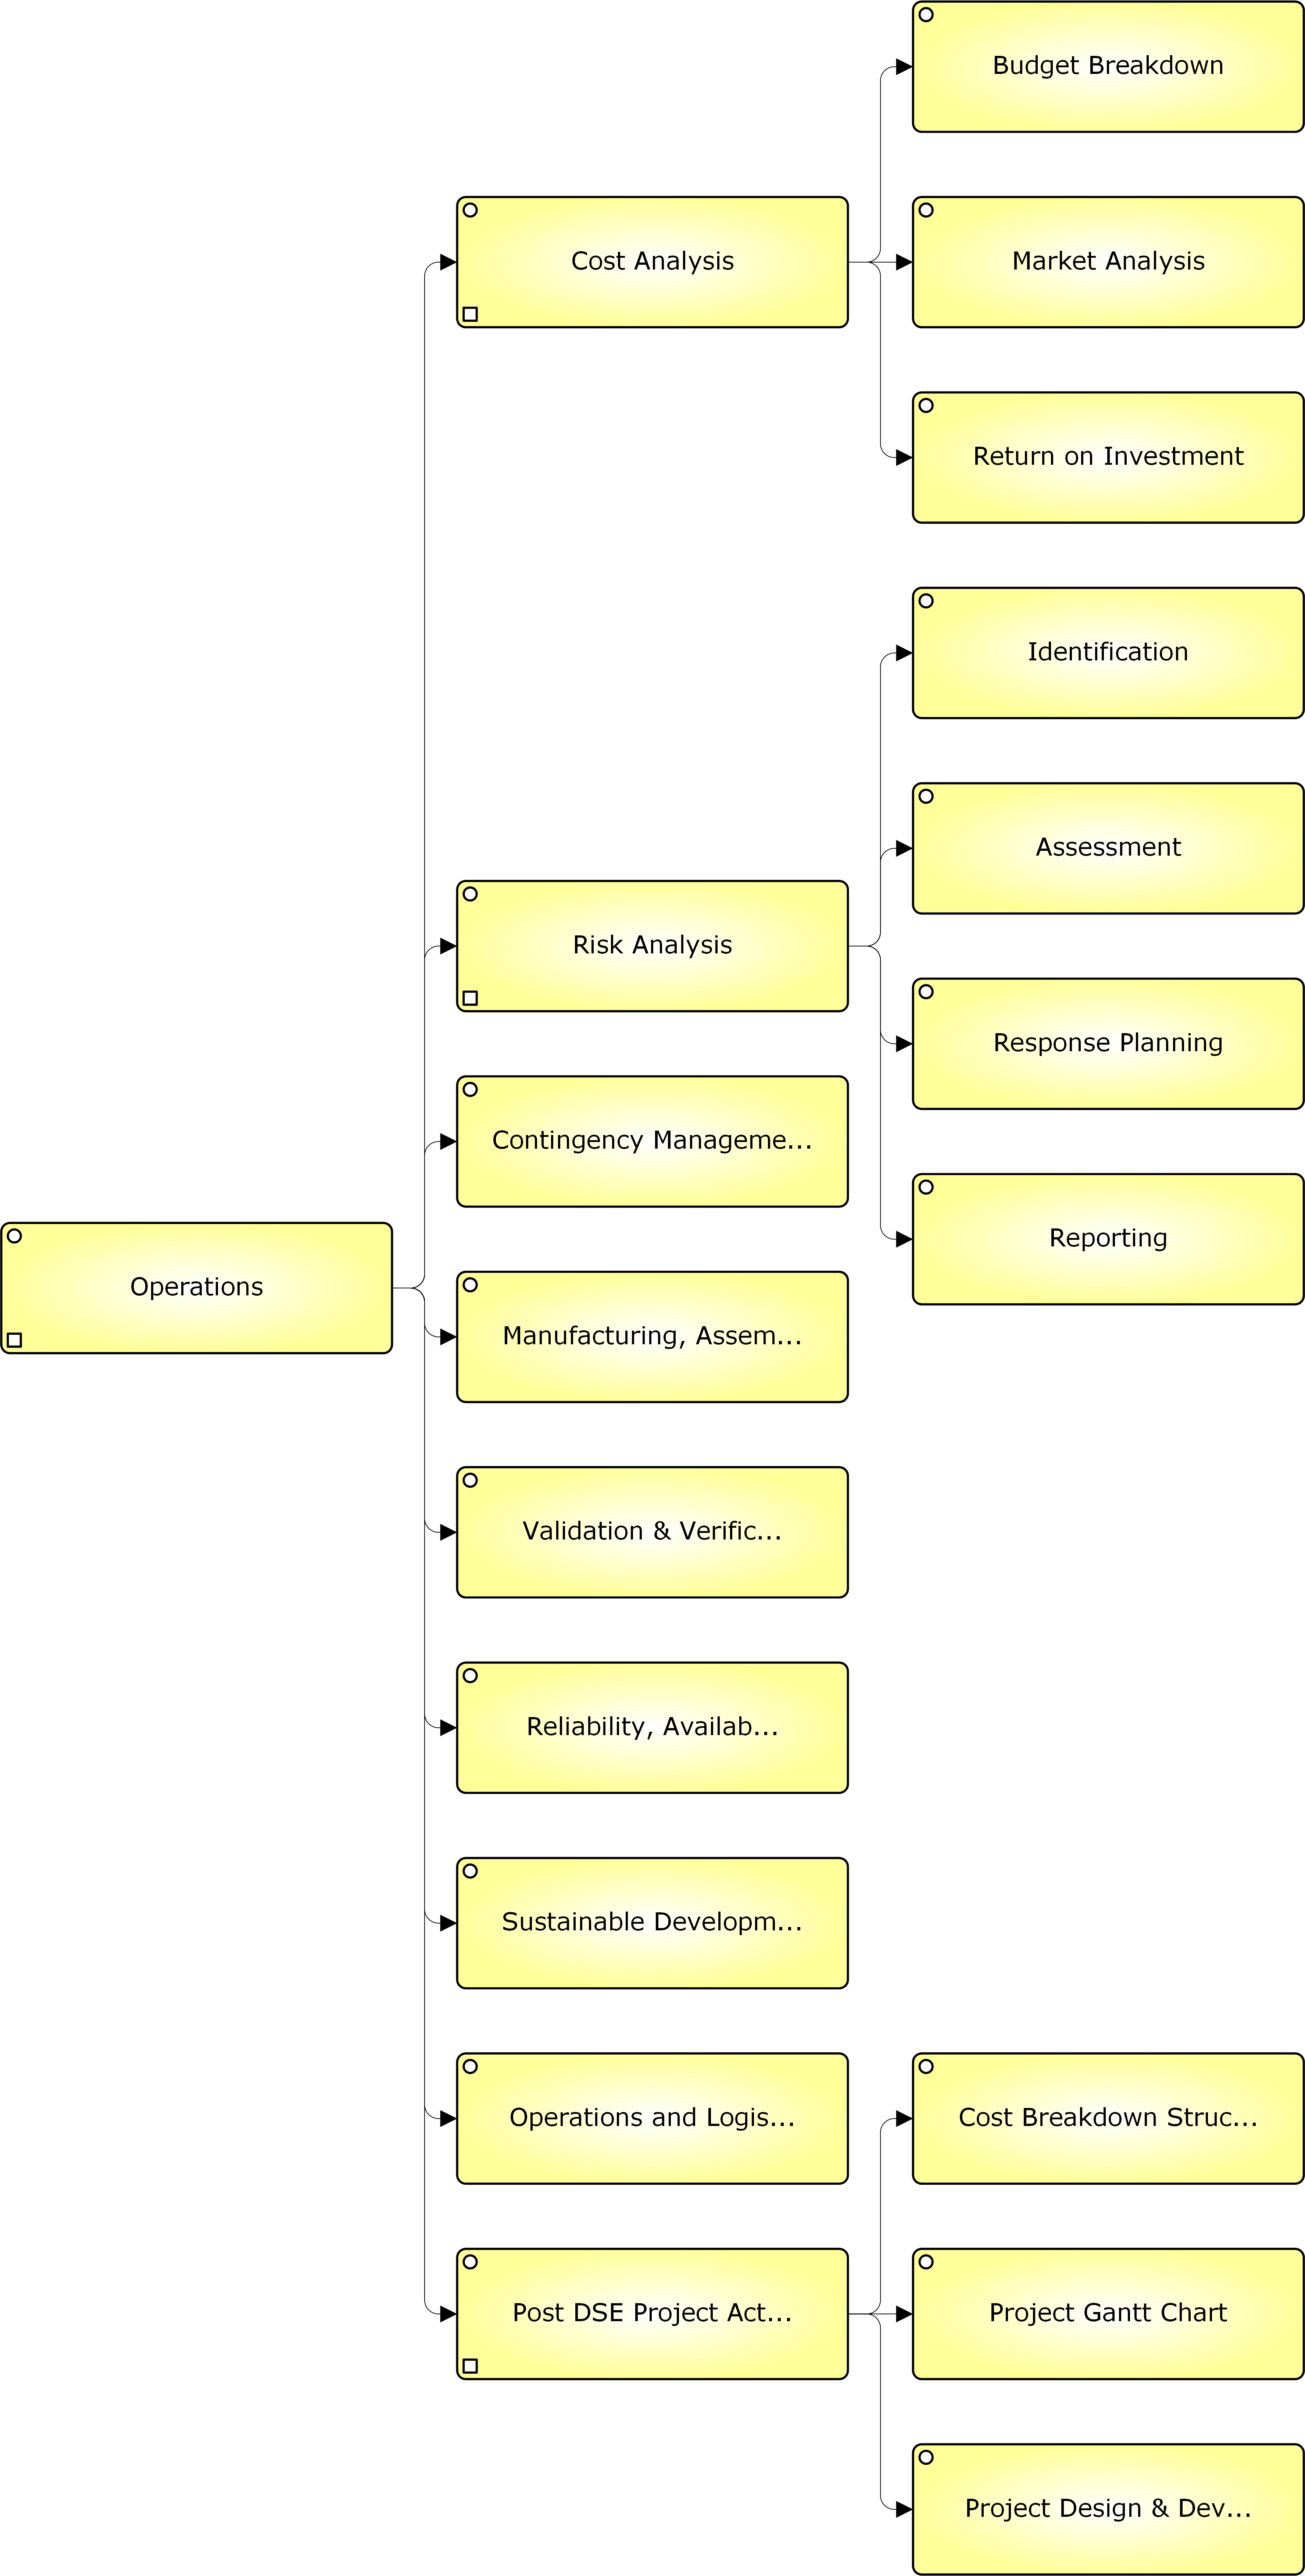
\includegraphics[height=20cm]{Figures/WBS_O.png}

\caption{operations WBS tree}
\end{figure}






\begin{figure}
\label{fig:WBSDP}
\centering
\includegraphics[height=20cm]{Figures/WBS_DP.png}

\caption{Design/Product WBS tree}
\end{figure}



\begin{figure}
\label{fig:WBSPW}
\centering
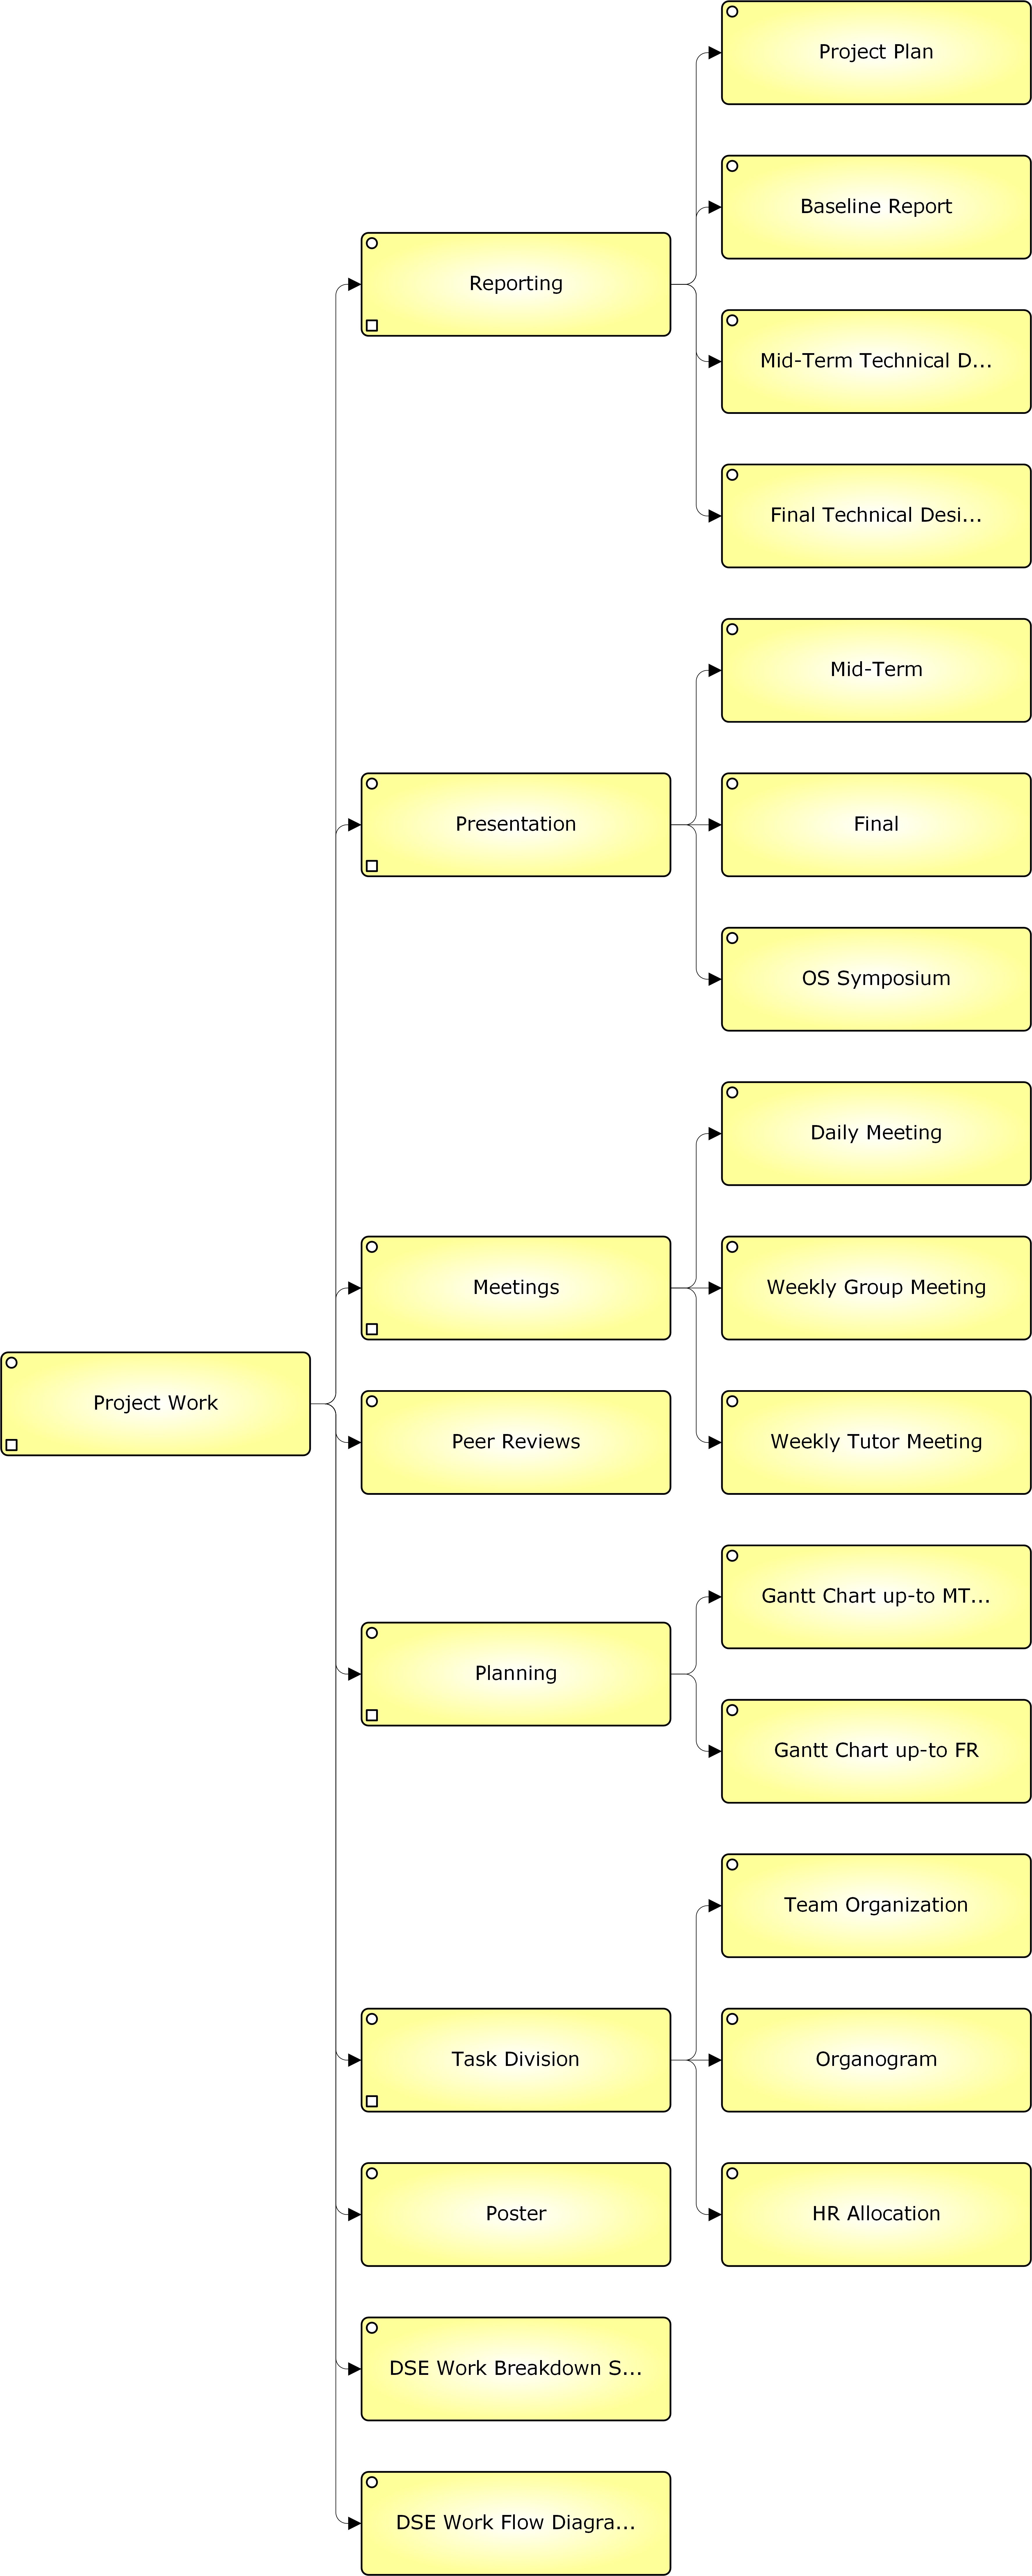
\includegraphics[height=20cm]{Figures/WBS_PW.png}

\caption{Project Work WBS tree}
\end{figure}



\end{document}